The circuit of the mixer was built according to figure[\ref{fig:clip}]. Two audio source was connect to $V_1$ and $V_2$, while a speaker was connected to $V_{out}$. The major difference between this mixer and that in lab2 is that one of the input is a microphone. We used a preamplifier introduced in section III-A to manage the input audio signal from microphone before it got mixed. We noticed that when the gain of the microphone reached a certain threshold, a high-frequency noise with high volume was generated. Controlling the volume of the microphone channel, we successfully mixed the audios. Beside the volume limitation of the microphone channel, the function of the potentiometers are just the same as what in the previous lab. 


\begin{figure*}[!htbp]
	\centering
	\begin{framed}
		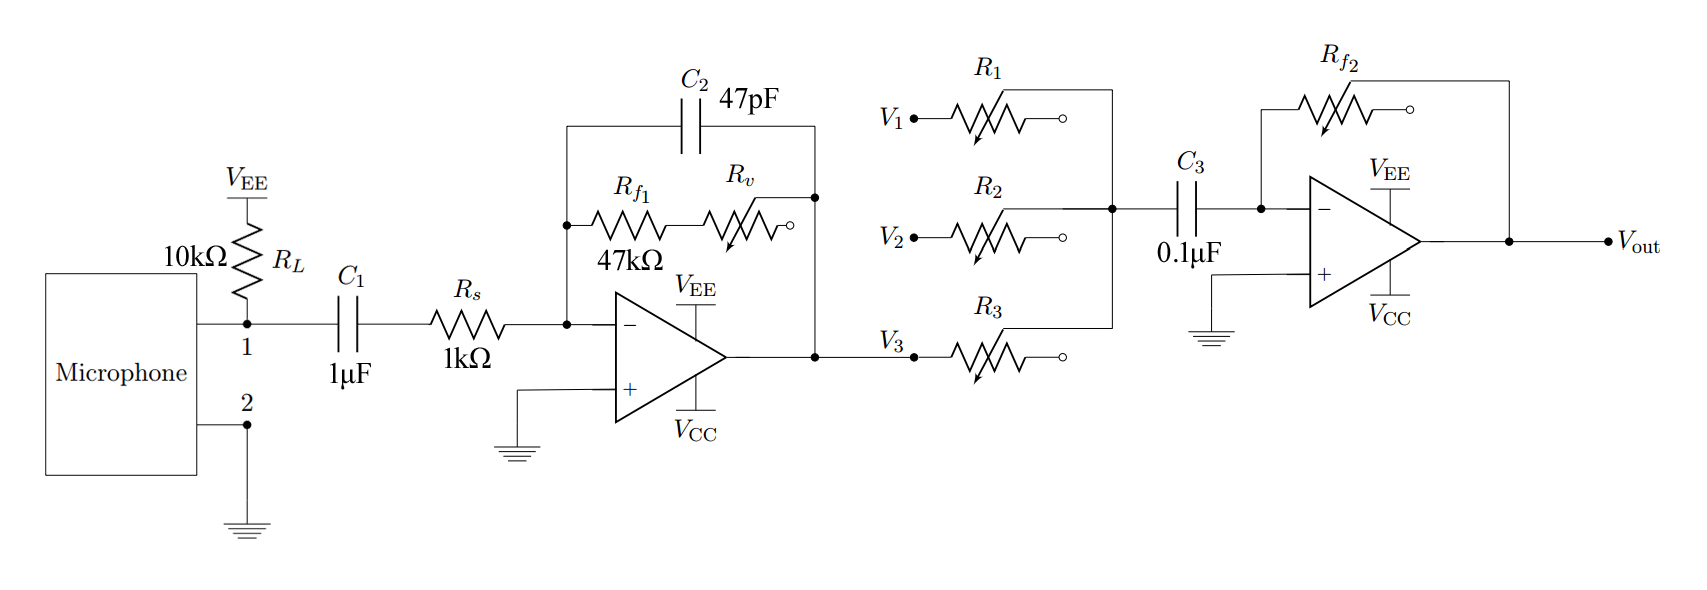
\includegraphics[width=\textwidth]{images/clip.png}
		\caption{The circuit of the mixer}
		\label{fig:clip}
	\end{framed}
\end{figure*}